% To familiarize yourself with this template, the body contains
% some examples of its use.  Look them over.  Then you can
% run LaTeX on this file.  After you have LaTeXed this file then
% you can look over the result either by printing it out with
% dvips or using xdvi.
%

\documentclass[twoside]{article}
%\usepackage{soul}
\usepackage{./lecnotes_macros}


\begin{document}
%FILL IN THE RIGHT INFO.
%\lecture{**LECTURE-NUMBER**}{**DATE**}{**LECTURERS**}{**SCRIBE**}
\lecture{3}{22 January 2025}{Maria Francis and M. V. Panduranga Rao}{Gautam Singh}
%\footnotetext{These notes are partially based on those of Nigel Mansell.}

%All figures are to be placed in a separate folder named ``images''

% **** YOUR NOTES GO HERE:

\section{Cryptanalysis of DES Reduced to 8 Rounds}
DES reduced to 8 rounds uses a 5-round characteristic with probability 
approximately \(\frac{1}{10486}\) as shown in \autoref{fig:des-8-char}.

\begin{figure}[!ht]
    \centering
    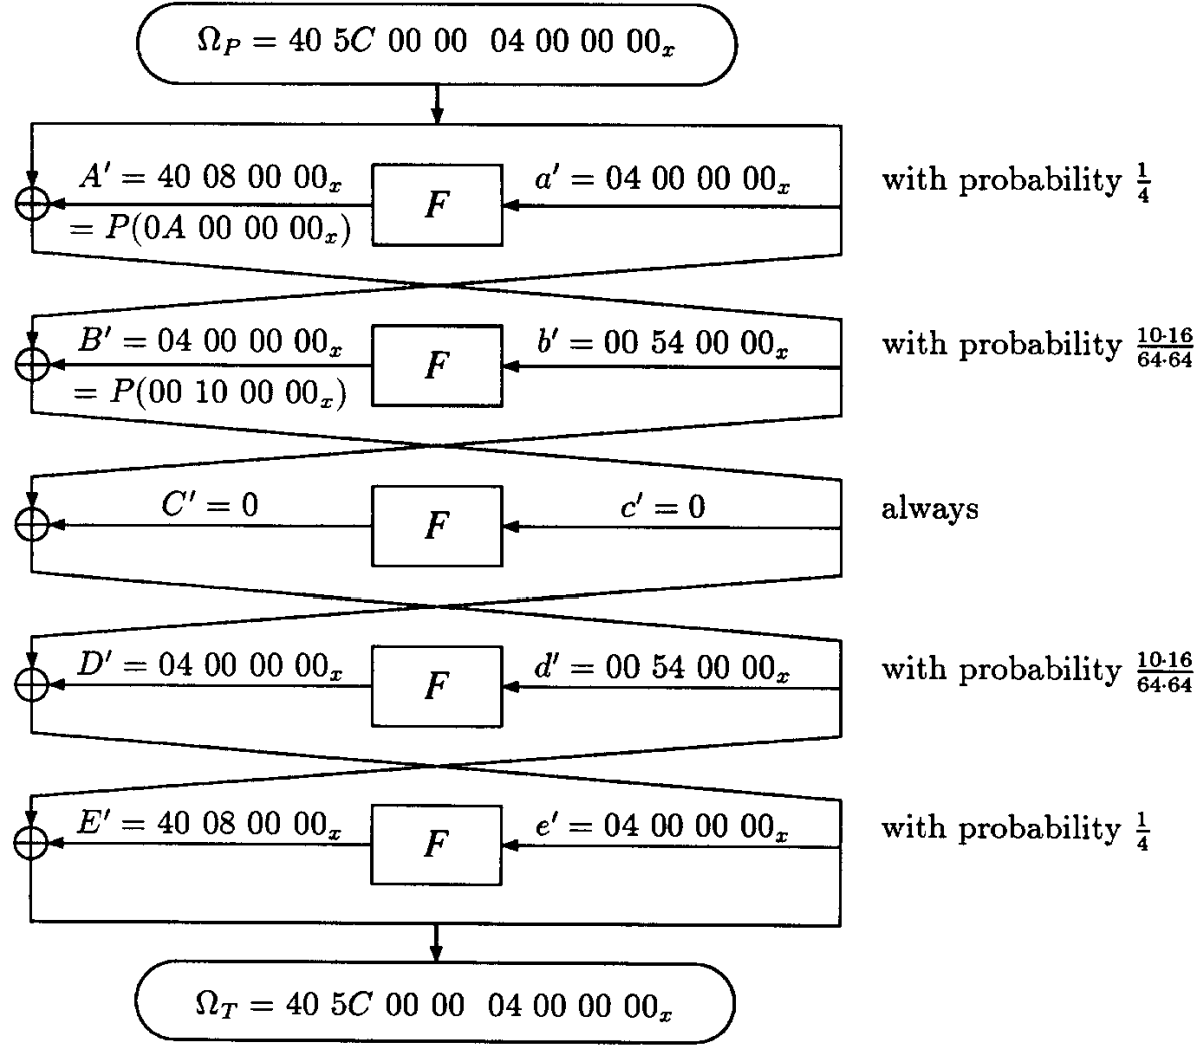
\includegraphics[width=0.5\textwidth]{images/des_8round_char.png}
    \caption{5 round characteristic used to cryptanalyze DES reduced to 8 rounds.}
    \label{fig:des-8-char}
\end{figure}

From the characteristic, it is evident that
\begin{equation}
    f^\prime = d^\prime \oplus E^\prime = b^\prime \oplus A^\prime = L^\prime = \texttt{40 5C 00 00}.
\end{equation}

Thus, for a right pair, five S boxes S2, S5, \dots, S8 have zero input XORs in
the sixth round. Using
\begin{equation}
    H^\prime = l^\prime \oplus g^\prime = l^\prime \oplus e^\prime \oplus F^\prime
\end{equation}

and the fact that \(h^\prime = r^\prime\), we can count on \(5 \cdot 6 = 30\)
key bits of \(K8\). The signal to noise ratio is \(S/N = \frac{2^{30}}{4^5 \cdot
10486} \approx 100\). However, due to the large memory requirement of \(2^{30}\)
locations, we count on fewer key bits. Further, due to the small probability of
the characteristic, we require many plaintexts, which makes the clique method
slow. Notice that each S box discards 20 \% of wrong pairs. Thus, counting on 24
key bits has \(S/N = \frac{2^{24}}{4^4 \cdot 0.8 \cdot 10486} \approx 7.8\) and
counting on 18 key bits has \(S/N = \frac{2^{18}}{4^3 \cdot 0.8^2 \cdot 10486}
\approx 0.6\).

\subsection{Modifying the Characteristic}
By reducing the number of key bits to count, we can also choose which key bits
are to be counted in order to improve the signal to noise ratio. Notice that

\begin{equation}
    e^\prime = \texttt{04 00 00 00} \rightarrow E^\prime = P\brak{\texttt{0W 00 00 00}} = \texttt{X0 0Y Z0 00}
    \label{eq:des-8-r5-rel}
\end{equation}

where \(W \in \cbrak{0,1,2,3,8,9,A,B},\ X,Z \in \cbrak{0,4},\ Y \in
\cbrak{0,8}\). Hence, we have \(f^\prime = d^\prime \oplus E^\prime = \texttt{X0
5V Z0 00}\) where \(V = Y \oplus 4\). If \(Z = 0\), then necessarily \(E^\prime
= \texttt{40 08 00 00}\) and this happens with probability \(\frac{16}{64}\).
All other combinations involving \(Z = 4\) occur with probability
\(\frac{20}{64}\).

Although we cannot count on \(S5_{Kh}\), one can check \(S5^\prime_{Eh}
\rightarrow S5^\prime_{Oh}\) which is satisfied by approximately 80 \% of the
pairs. Thus, the modified probability of \(e^\prime \rightarrow E^\prime\) is
\(\frac{16}{64} + 0.8\frac{20}{64} = \frac{1}{2}\). This doubles the probability
of the characteristic \(\Omega_P\) to \(\frac{1}{5243}\) and consequently
doubles the \(S/N\) for counting on 24 bits and 18 bits of \(K8\) to \(15.6\)
and \(1.2\) respectively.

\end{document}
